%%%%%%%%%%%%%%%%%%%% author.tex %%%%%%%%%%%%%%%%%%%%%%%%%%%%%%%%%%%
%
% sample root file for your "contribution" to a proceedings volume
%
% Use this file as a template for your own input.
%
%%%%%%%%%%%%%%%% Springer %%%%%%%%%%%%%%%%%%%%%%%%%%%%%%%%%%
\documentclass[hidelinks]{svproc}
%
% RECOMMENDED %%%%%%%%%%%%%%%%%%%%%%%%%%%%%%%%%%%%%%%%%%%%%%%%%%%
%
% to typeset URLs, URIs, and DOIs
\usepackage{url}
\def\UrlFont{\rmfamily}
\usepackage{graphicx}

\def\ingles{}

\ifdefined\ingles
	\usepackage{babel}
\else
	\usepackage[spanish]{babel}
\fi
\usepackage{hyperref}
% Microtype tiene que preceder a Ragged2e
\usepackage[babel=true,expansion=true,protrusion=true]{microtype}
% Ragged2e tiene que ir despues de microtype para funcionar correctamente sino cambia las alineaciones y no quedan bien
\usepackage{ragged2e}
%----------------------------------------------------------------------------------------
%	BIBLIOGRAPHY AND INDEX
%----------------------------------------------------------------------------------------
\usepackage[
	%style=splncs03,
	%style=IEEEtran,
	style=nature,
	citestyle=numeric,
	%sorting=none,
	%sortcites=true,
	%autopunct=true,
	babel=hyphen,
	hyperref=true,
	abbreviate=false,
	%backref=true,
	backend=biber,
	bibencoding=utf8,
	defernumbers=true
]{biblatex}

% MARCAS DE AGUA
%\usepackage{draftwatermark}
%\SetWatermarkColor{gray!20}
%\SetWatermarkText{PRELIMINAR}
%\SetWatermarkScale{3}

% TO DO LIST
%\usepackage[colorinlistoftodos,textsize=tiny]{todonotes}

\usepackage{float}
%\newcommand{\cita}{\footnote{Se necesita cita}}

\newcommand{\revisar}[1]{\todo[backgroundcolor=yellow!50]{#1}}
\newcommand{\ampliar}{\todo[backgroundcolor=blue!30]{Ampliar}}
\newcommand{\cita}{\todo[backgroundcolor=red!50]{\textbf{FALTA CITA}}}
\newcommand{\figura}{\missingfigure{Falta figura\ldots}}

\defbibheading{bibempty}{}
\DeclareBibliographyCategory{cited}
\AtEveryCitekey{\addtocategory{cited}{\thefield{entrykey}}}
\nocite{*}

\bibliography{./bib/refs} % ESTE ANDA

\ifdefined\peerreview
	\newcommand{\utn}{\colorbox{lightgray}{OCULTO PARA BLIND REVIEW}}
	\newcommand{\frc}{\colorbox{lightgray}{OCULTO PARA BLIND REVIEW}}
	\newcommand{\cids}{\colorbox{lightgray}{OCULTO PARA BLIND REVIEW}}
	\newcommand{\depto}{\colorbox{lightgray}{OCULTO PARA BLIND REVIEW}}
\else
	\newcommand{\utn}{Universidad Tecnológica Nacional}
	\newcommand{\frc}{Facultad Regional Córdoba }
	\newcommand{\cids}{CIDS – Centro de Investigación, Desarrollo y Transferencia en Sistemas de Información}
	\newcommand{\depto}{Departamento de Ingeniería en Sistemas de Información}
\fi

\begin{document}
\mainmatter              % start of a contribution
%
\ifdefined\ingles
	\title{Graph databases as storage support for detection of star clusters in nearby galaxies}
	\titlerunning{Graph data bases as storage support\ldots}
\else
	\title{Bases de datos de grafos como soporte para la detección de estrellas jóvenes en cúmulos estelares cercanos}
	\titlerunning{Bases de datos de grafos como soporte\ldots}
\fi
%
%\titlerunning{Bases de datos de grafos\ldots}  % abbreviated title (for running head)
%                                     also used for the TOC unless
%                                     \toctitle is used
%
\author{
	Martín Casatti\inst{1},
	Analía Guzmán\inst{1},
	María Alejandra Paz Menvielle\inst{1}
}
%
\authorrunning{Casatti M., Guzmán A., Paz Menvielle M.} % abbreviated author list (for running head)
%
%%%% list of authors for the TOC (use if author list has to be modified)
\tocauthor{Casatti M., Guzmán A., Paz Menvielle M.}
%
\institute{Universidad Tecnológica Nacional - Facultad Regional Córdoba, Córdoba, Argentina,\\
\email{mcasatti@frc.utn.edu.ar, aguzman@frc.utn.edu.ar,pazmalejandra@gmail.com}}

\maketitle              % typeset the title of the contribution

\begin{abstract}
	% Planteo de un abstract estructurado. Las secciones (aunque no se coloquen explícitamente) son:
	% Background
	% Aim: Objetivo del trabajo
	% Method: Método que se utilizó para hacer el trabajo
	% Results: Resultados
	% Conclusion: Conclusiones
\ifdefined\ingles
	The present work will explore the most outstanding features that a graph database should gather for the implementation of a system for structural patterns recognition in nearby star clusters.
	The parameters to be stored will be analyzed, according to the information revealed by various astronomical observation projects, as well as the most promising representation model, considering the purpose of storage.
	Some of the characteristics of existing databases will also be described, as well as their advantages and disadvantages when implementing the recognition system.
	It will be demonstrated that a representation in the form of graphs of the existing information in the astronomical repositories is not only possible and can help to the automatic processing  but also can provide an effective mechanism for the implementation of pattern recognition algorithms and the consequent detection of stellar structures of interest.
\else
	El presente trabajo explorará las características más destacadas que debe reunir una base de datos de grafos para la implementación de un sistema de reconocimiento de patrones estructurales en cúmulos estelares cercanos. Se analizarán los parámetros a almacenar, de acuerdo a la información relevada por diversos proyectos de observación astronómica, así como el modelo de representación más prometedor, considerando la finalidad del almacenamiento. Se describirán también algunas de las características de bases de datos existentes, así como sus ventajas y desventajas a la hora de implementar el mencionado sistema de reconocimiento.
	Se demostrará que una representación en forma de grafos de la información existente en los repositorios astronómicos no sólo es posible y puede ayudar al procesamiento automático de dicha información sino que además puede proveer un mecanismo efectivo para la implementación de algoritmos de reconocimiento de patrones y la consecuente detección de estructuras estelares de interés.
\fi
\ifdefined\ingles
	\keywords{graph, database, modeling, pattern detection, astronomy, stellar clusters}
\else
	\keywords{grafos, base de datos, modelado, detección de patrones, astronomía, cúmulos estelares}
\fi
\end{abstract}


\section{
\ifdefined\ingles	
	Context
\else
	Contexto
\fi
}
\ifdefined\ingles	
	This report is part of the work aimed at developing a master's thesis for obtaining the title of Master in Information Systems Engineering, which seeks to determine the effectiveness of algorithms based on graphs for the detection of structural patterns in models of astronomical systems, specifically with regard to star clusters in nearby galaxies.
	
	The aforementioned thesis is developed in the context of a research and development project that has been approved by the Secretaría de Investigación, Desarrollo y Posgrado, in the \utn, which is carried out in the \cids.
	
	At present there is a large amount of information from nearby galaxies due, in large part, to the fact that the Hubble Space Telescope (HST) has allowed obtaining data with high spatial resolution using several wide-field cameras (WFPC2, ACS) \cite{dalcanton2009acs}. This access facilitates research linked to stellar groups, on different populations and histories of star formation.
	
	It has long been recognized in the field of astrophysics that stellar clusters are important laboratories for research, since they contain statistically significant samples of stars of approximately the same age in a small space. On the other hand, the stellar groups existing in them provide valuable information for the understanding of the structure of the galaxy that contains them.
	
	There is currently a huge amount of information obtained from continuous observation projects, mainly in survey mode\cite{borne2008scientific, frinchaboy2012sdss} such as:
	
	\begin{itemize}
		\item VVV\cite{minniti2010vista} (\url{https://vvvsurvey.org/})
		\item LSST\cite{ivezic2007astrometry} (\url{https://www.lsst.org/})
		\item SDSS\cite{bundy2014overview} (\url{https://www.sdss.org/})
		\item Gaia-ESO\cite{gilmore2012gaia} (\url{https://www.gaia-eso.eu/})
	\end{itemize}

	All the mentioned examples require automatic mechanisms for the analysis of data.

	The Data Minning (DM) algorithms, in particular those related to the automatic pattern recognition, are currently having an important revision and development\cite {borne2009astroinformatics, ball2010data, schmeja2011identifying} for their application on the data that arise from the big surveys.
	
	In this work we intend to expose the capabilities of the graph databases to support algorithms for automatic pattern recognition on astronomical data. The aim is to determine if these techniques, from other fields of application, are transferable to the field of astronomy, with or without adjustments, or if the information from astronomical databases requires recognition algorithms designed specifically for them.
	
	In a first stage, the way in which the preprocessing and data acquisition will be performed will be analyzed, to then carry out the stages of extraction of the fundamental characteristics and the grouping or classification to achieve the identification and parameterization of new stellar groups.
	
	Regarding the preprocessing and acquisition of data, it will be described how the selected data model is and how, from the sample of data obtained from the optical instruments, it will be prepared to store it in a graph, in order to continue with the detection and recognition stages of related patterns.
\else
	El presente informe forma parte de los trabajos orientados a la elaboración de una tesis de maestría para la obtención del título de Magister en Ingeniería en Sistemas de Información, la cual busca determinar la efectividad de algoritmos basados en grafos para la detección de patrones estructurales en modelos de sistemas astronómicos, específicamente en lo que respecta a cúmulos estelares en galaxias cercanas.
	
	La mencionada tesis se desarrolla en el marco de un proyecto de investigación y desarrollo que ha sido homologado por la Secretaría de Investigación, Desarrollo y Posgrado de la \utn, el cual se lleva a cabo en el ámbito del \cids.
	
	En la actualidad existe una gran cantidad de información de las galaxias cercanas debido, en gran parte, a que el Telescopio Espacial Hubble (HST) ha permitido obtener datos con alta resolución espacial utilizando varias cámaras de campo amplio (WFPC2, ACS)\cite{dalcanton2009acs}. Este acceso facilita realizar investigaciones vinculadas con agrupaciones estelares, sobre diferentes poblaciones e historias de formación estelar.
	
	Desde hace tiempo se reconoce en el campo de la astrofísica que los cúmulos estelares son laboratorios importantes para la investigación, ya que contienen muestras estadísticamente significativas de estrellas de aproximadamente la misma edad en un espacio reducido. Por otra parte, las agrupaciones estelares existentes en los mismos brindan información valiosa para la comprensión de la estructura de la galaxia que las contiene. 
	
	Existe actualmente una enorme cantidad de información obtenida a partir de proyectos de observación continua, principalmente en modo “survey”\cite{borne2008scientific,frinchaboy2012sdss} como pueden ser:
	\begin{itemize}
		\item VVV\cite{minniti2010vista} (\url{https://vvvsurvey.org/})
		\item LSST\cite{ivezic2007astrometry} (\url{https://www.lsst.org/})
		\item SDSS\cite{bundy2014overview} (\url{https://www.sdss.org/})
		\item Gaia-ESO\cite{gilmore2012gaia} (\url{https://www.gaia-eso.eu/})
	\end{itemize}
	
	Todos los ejemplos mencionados requieren de mecanismos automáticos para el análisis de los datos.
	
	Los algoritmos de “Data Mining” (DM), en particular los relacionados con el reconocimiento automático de patrones, están en la actualidad teniendo una importante revisión y desarrollo\cite{borne2009astroinformatics,ball2010data,schmeja2011identifying} para su aplicación sobre los datos que surgen de los grandes “surveys”. 
	
	En este trabajo se pretende exponer las capacidades de las bases de datos de grafos para soportar algoritmos de reconocimiento automático de patrones sobre datos astronómicos. Se busca determinar si dichas técnicas, provenientes de otros ámbitos de aplicación, son trasladables al ámbito de la astronomía, si se requieren o no adecuaciones, o si la información de las bases de datos astronómicos requiere de algoritmos de reconocimiento diseñados específicamente para las mismas.
	
	En una primera etapa se analizará la forma en que se realizará el preprocesamiento y adquisión de datos, para luego realizar las etapas de extracción de las características fundamentales y el agrupamiento o clasificación para lograr la identificación y parametrización de nuevas agrupaciones estelares.
	
	Respecto al preprocesamiento y adquisión de datos se describirá como es el modelo de datos seleccionado y como a partir de la muestra de datos obtenida del instrumental óptico, se lo preparara para almacenarlo en un grafo, para luego poder continuar con las etapas de detección y reconocimiento de patrones relacionados.
\fi


\section{
\ifdefined\ingles	
	Introduction
\else
	Introducción
\fi
}
\ifdefined\ingles	
	A pattern is an entity that can be given a name and that is represented by a set of measured properties and the relationships between them are represented in the so-called \emph{feature vector}\cite{watanabe1985pattern}.
	
	In the domain of astronomical data a pattern can be the average distances between stars of the same cluster, their spectral characteristics, their brightness curve, etc. The vector of characteristics would be formed, in this case, by physical, chemical or structural characteristics that relate the different elements.
	
	There are works that have focused on improving the knowledge of our own Galaxy and the Magellanic Clouds, for example Baume et al. 2008\cite{baume2008basic}, but currently there are several factors that significantly increase the number of objects to analyze, making an automatic method for data processing especially relevant.
	
	The automatic recognition, description, classification and grouping of patterns are important activities in a great variety of scientific disciplines, such as biology, psychology, medicine, computer vision, artificial intelligence, remote sensing, etc. The main importance of pattern detection in the data is that you can infer causes for the grouping of the data and this is where the interest of the application of these techniques to the astronomical field lies.
	
	Although currently there are research lines studying recognition methods based on vector support machines\cite{burges1998tutorial} the approach used in this research line focuses on the structural characteristics of the graphs\cite{bunke1983inexact, pavlidis2013}.
	
	The following are fundamental concepts related to the construction of graphs:
	
	\textbf{Node:} A node is a \emph{information entity} different from any other entity in the model. All nodes represent a single set of information which is indivisible and independent of any other information represented. Larger units can be represented only as groups of related nodes. For the purposes of this project, it is necessary that each node can be uniquely and differently identified from all other nodes in the network.
	
	\textbf{Link:} A link is used to establish a relationship between two nodes of the model.
	A link can only connect two nodes. One called \emph{origin} from which the link exits and one called \emph{destination} to which it arrives. A relationship between a source node and two destination nodes requires two links, both with the same origin, but with different destinations. A node can be the source of several links, as well as the destination of several links\cite{van2010graph, bondy1976graph}.
	
	\subsection{Patterns in Graphs}
	
	The recognition or detection of patterns within graphs seeks to detect a subgraph (pattern) in a graph (objective). We must consider that this search for coincidences can be broken down into two parts:
	
	\begin{enumerate}
		\item A structural match, where the nodes and relations of the pattern make up an existing structure in the objective graph.
		\item A match at the level of elements, where the nodes and relations, at the level of their particular attributes, have the same values as in the structure found in the objective graph.
	\end{enumerate}

	Many times the search for these two matches is executed separately to optimize the algorithms or reduce the search space\cite{fan2012graph}.
	
	In the domain under study, the detection of a subgraph (pattern) will be performed on the graphs generated from astronomical information provided by continuous observation files (survey) such as those found in the VVV Survey project, the Large Scale Telescope (LST) project or Hubble Space Telescope (HST) project, the latter being the origin of data that will be used in this and subsequent works.
	
	\subsection{Metrics in graphs}
	
	A tool widely used to describe graphs and often used to start the analysis of existing patterns in them, is the calculation of local or global metrics\cite{van2010graph}, which allow to characterize the objective graph or the base graph. The metrics can be divided into two large groups:
	
	\begin{itemize}
		\item Static Metrics: When they are calculated on a static graph at a given point in time. They focus mainly on the structural characteristics of it.
		\item Dynamic metrics: They take into account the temporal dimension of the changes that occur on the graph. They are more focused on the variations between two instants of time, rather than on the characteristics of the graph in each one of those instants.
	\end{itemize}

	Another approach to the analysis of the metrics is to analyze on which components of the graph the measurements are made. From this point of view there are different perspectives, the most common being:

	\begin{itemize}
		\item Network metrics (or global): Metrics that take as a reference the complete graph, with all the nodes and arcs that comprise it.
		\item Node metrics (or local): Are those that take as reference a node or subset of nodes to perform the calculations.
	\end{itemize}

	Here are some common metrics:
	
	\subsubsection{Global metrics:}
	
	Centrality: This metric tries to determine which node or nodes occupy a central location in the network, being equidistant from the other nodes.
	
	Connection: It seeks to establish the degree to which the nodes of a graph are connected with all the other nodes of the same graph. You can find, by applying this metric, strongly connected or weakly connected components.
	
	Number of Components: In a graph that is not completely connected, it indicates the number of related subgraphs that are part of the graph. A component is a set of connected nodes that are part of the main graph.
	
	Size of the giant component: It measures the number of nodes that the connected component has that is greater than all the other components of the graph. In a connected graph the size of the giant component is equal to the total number of nodes.
	
	Shortest/longest route: Express the minimum/maximum length (in arcs) between two given nodes.
	
	\subsubsection {Local metrics:}
	
	Connectivity: Expresses the number of connections a specific node has. It can be expressed as 'degree', if it does not take into account the direction of the arcs that impinge or leave the node, or as 'input degree' or 'output degree' when only taking into account incoming or outgoing arcs, respectively .
	
	Centrality: It is a metric, associated with a node in a graph, which determines its relative importance within it, and can be divided into:
	
	\begin{itemize}
		\item Centrality of degree: Number of connections with other nodes
		\item Centrality of proximity: Indicates how close one unit is to the network of others.
		\item Intermediation centrality: Indicates whether a unit is within some of the shortest routes between two nodes in the network.
	\end{itemize}

	\subsection{Pattern recognition design}

	The main objective of a automatic pattern recognition system is to discover the underlying nature of a phenomenon or object, describing and selecting the fundamental characteristics that allow them to be classified in a certain category\cite{batagelj2006data,fukunaga2013introduction}.

	Automatic pattern recognition systems allow addressing problems in computer science, engineering and other scientific disciplines \cite{devijver2012pattern,meyer2004pattern}, therefore the design of each stage requires joint analysis criteria to validate the results\cite{kim2005robust,kim2005new}.

	After analyzing different ways of designing a pattern recognition system, we consider three phases\cite{alonso2001redes}:
	
	\begin{enumerate}
		\item Acquisition and preprocessing of data.
		\item Feature extraction.
		\item Decision making or grouping.
	\end{enumerate}
	
	In the data acquisition and pre-processing phase, the database infrastructure will be prepared in order to continue with the following phases.
	
	For the next two phases, feature extraction and decision making or grouping the most relevant parameters that make up stellar groups of interest will be considered, working in collaboration with experts from the Instituto Astrofísico de La Plata, Buenos Aires, Argentina.
\else
	Un patrón es una entidad a la que se le puede dar un nombre y que está representada por un conjunto de propiedades medidas y las relaciones entre ellas representadas en el denominado \emph{vector de características}\cite{watanabe1985pattern}. 
	
	En el dominio de los datos astronómicos un patrón puede ser las distancias medias entre estrellas del mismo cúmulo, sus características espectrales, su curva de luminosidad, etc. El vector de características estaría conformado, en este caso, por características físicas, químicas o estructurales que relaciones los distintos elementos.
	
	Existen trabajos que se han focalizado en mejorar el conocimiento de nuestra propia Galaxia y de las Nubes de Magallanes, por ejemplo Baume et al. 2008\cite{baume2008basic}, pero actualmente hay varios factores que incrementan de forma importante tanto la cantidad de objetos a analizar tornando especialmente relevante un método automático para el procesamiento de los datos.
	
	El reconocimiento automático, descripción, clasificación y agrupamiento de patrones son actividades importantes en una gran variedad de disciplinas científicas, como biología, psicología, medicina, visión por computador, inteligencia artificial, teledetección, etc. La principal importancia que tiene la detección de patrones en los datos es que se pueden inferir causas para la agrupación de los mismos y es aquí donde radica el interés de la aplicación de éstas técnicas al ámbito astronómico.
	
	%Este trabajo, tiene paralelos con el llamado SNA (Social Network Analysis, Análisis de Redes Sociales) que es una disciplina cuyo objetivo es:
	%
	%\begin{quote}
	%\emph{``Analizar la estructura de una red social para \textbf{inferir conocimiento} de un individuo, un grupo, o las relaciones entre ellos''}\cite{scott2011sage}.	
	%\end{quote}
	
	Si bien actualmente se están investigando métodos de reconocimiento basados en máquinas de soporte vectorial\cite{burges1998tutorial} el enfoque utilizado en la presente línea de investigación se centra en las características estructurales de los grafos\cite{bunke1983inexact,pavlidis2013}.
	
	Se describen a continuación conceptos fundamentales relacionados a la construcción de grafos:
	
	\textbf{Nodo:} Un nodo es un \emph{entidad de información} diferente de cualquier otra entidad en el modelo. Todos los nodos representan un único conjunto de información la cual es indivisible e independiente de cualquier otra información representada. Unidades mayores pueden representarse únicamente como grupos de nodos relacionados.Para los fines que se persiguen es necesario que cada nodo pueda ser identificado de manera unívoca y diferente de todos los demás nodos de la red.
	
	\textbf{Enlace:} Un enlace se utiliza para establecer una relación entre dos nodos del modelo. 
	Un enlace solo puede conectar dos nodos. Uno denominado \emph{origen} desde el que sale el enlace y uno denominado \emph{destino} al cual llega. Una relación entre un nodo de origen y dos nodos de destino requiere de dos enlaces, ambos con el mismo origen, pero con diferentes destinos. Un nodo puede ser origen de varios enlaces, así como puede ser destino de varios enlaces\cite{van2010graph,bondy1976graph}.
	
	\subsection{Patrones en Grafos}
	
	El reconocimiento o detección de patrones dentro de grafos busca detectar un subgrafo (patrón) en un grafo (objetivo). Debemos considerar que esta búsqueda de coincidencias se puede descomponer en dos partes:
	
	\begin{enumerate}
		\item Una concordancia estructural, en donde los nodos y relaciones del patrón conforman una estructura existente en el grafo objetivo.
		\item Una concordancia a nivel de elementos, en donde los nodos y relaciones, a nivel de sus atributos particulares, tiene los mismos valores que en la estructura encontrada en el grafo objetivo.
	\end{enumerate}
	
	Muchas veces la búsqueda de estas dos concordancias se ejecuta de forma separada para optimizar los algoritmos o reducir el espacio de búsqueda\cite{fan2012graph}.
	
	En el dominio bajo estudio la detección de un subgrafo (patrón) se realizará sobre los grafos generados a partir de información astronómica suministrada por archivos de observación continua (survey) tales como los encontrados en los proyectos VVV Survey, Large Scale Telescope (LST) o Hubble Space Telescope (HST), siendo éste último el origen de los datos que se van a utilizar en éste y sucesivos trabajos.
	
	\subsection{Métricas en grafos}
	
	Una herramienta ampliamente utilizada para describir grafos y que muchas veces se utiliza para iniciar el análisis de patrones existentes en los mismos, es el cálculo de métricas\cite{van2010graph}, locales o globales, que permiten caracterizar el grafo objetivo o el grafo patrón. Las métricas se pueden dividir en dos grandes grupos:
	
	\begin{itemize}
		\item Métricas estáticas: Cuando se calculan sobre un grafo estático en un punto en el tiempo determinado. Se enfocan principalmente en las características estructurales del mismo.
		\item Métricas dinámicas: Tienen en cuenta la dimensión temporal de los cambios que se producen sobre el grafo. Están más enfocadas en las variaciones entre dos instantes de tiempo, antes que en las características propias del grafo en cada uno de esos instantes.
	\end{itemize}
	
	Otro enfoque para el análisis de las métricas radica en analizar sobre qué componentes del grafo se realizan las mediciones. Desde este punto de vista se tienen diversas perspectivas, siendo las más comunes:
	
	\begin{itemize}
		\item Métricas de redes (o globales): Son las métricas que toman como referencia el grafo completo, con todos los nodos y arcos que lo conforman.
		\item Métricas nodos (o locales): Son aquellas que toman como referencia un nodo o subconjunto de nodos para realizar los cálculos.
	\end{itemize}
	
	A continuación, se detallan algunas métricas más comunes:
	
	\subsubsection{Métricas globales:}
	
	Centralidad: Esta métrica trata de determinar que nodo o nodos ocupan una ubicación central en la red, estando equidistante de los demás nodos.
	
	Conexionado: Busca establecer el grado en el que los nodos de un grafo están conectados con todos los demás nodos del mismo. Se puede encontrar, aplicando esta métrica, componentes fuertemente conectados o débilmente conectados.
	
	Cantidad de Componentes: En un grafo que no es completamente conexto, indica la cantidad de subgrafos conexos que forman parte del grafo. Un componente es un conjunto de nodos conectados que forman parte del grafo principal.
	
	Tamaño del componente gigante: Mide la cantidad de nodos que tiene el componente conectado que es mayor que todos los demás componentes del grafo. En un grafo conexo el tamaño del componente gigante es igual a la cantidad total de nodos.
	
	Ruta más corta/larga: Expresa la longitud (en arcos) mínima/máxima entre dos nodos dados. 
	
	\subsubsection{Métricas locales:}
	
	Conectividad: Expresa la cantidad de conexiones que posee un nodo determinado. Se puede expresar como ‘grado’, si no tiene en cuenta la dirección de los arcos que inciden o salen del nodo, o como ‘grado de entrada’ o ‘grado de salida’ cuando solamente tiene en cuenta los arcos entrantes o salientes, respectivamente.
	
	Centralidad: Es una métrica, asociada a un nodo en un grafo, que determina su importancia relativa dentro de éste, pudiendo dividirse en:
	
	\begin{itemize}
		\item Centralidad de grado: Cantidad de conexiones con otros nodos
		\item Centralidad de cercanía: Indica qué tan cerca se encuentra una unidad de la red de otras.
		\item Centralidad de intermediación: Indica si una unidad se encuentra dentro de algunas de las rutas más cortas que existen entre dos nodos de la red.
	\end{itemize}
	
	%\subsection{Análisis de Patrones}
	%
	%\revisar{CAMBIAR ESTO}
	%
	%El análisis de patrones en el dominio bajo estudio, puede determinar si existen ciertos patrones que, aún, no siendo comunes en otras áreas de la teoría de grafos, si lo son recurrentes en este dominio. Se pueden determinar si son patrones temporales, es decir que tiendan a desaparecer en el tiempo a medida que la base de conocimientos va cambiando, o si son patrones permanentes y/o que se van reforzado con el tiempo.
	%
	%Dicho análisis puede servir para descubrir algunas características importantes que se relacionan con el aprendizaje, entre ellas:
	%
	%\begin{itemize}
	%	\item los temas que revisten más dificultad de aprendizaje,
	%	\item la cantidad y tipos de errores más comunes y su relación con el tema o concepto evaluado,
	%	\item las tendencias de los alumnos al momento de responder las mismas preguntas, es decir, si lo hacen con los mismos conceptos o, por el contrario, tienen una riqueza expresiva alta.
	%	\item Se propone incluir una respuesta textual, utilizada como patrón, para poder determinar si las respuestas dadas por los alumnos tienen una correspondencia directa (literal) con respecto al material brindado para su estudio.
	%\end{itemize}
	
	
	\subsection{Diseño de reconocimiento de patrones}
	
	El objetivo principal de un sistema de reconocimiento  automático  de  patrones  es  descubrir  la  naturaleza  subyacente  de  un  fenómeno u objeto, describiendo y seleccionado las características fundamentales que permitan  clasificarlos  en  una  categoría  determinada\cite{batagelj2006data}\cite{fukunaga2013introduction}.  
	
	Sistemas  automáticos  de  reconocimiento  de  patrones  permiten  abordar problemas  en  informática,  en  ingeniería  y en otras disciplinas científicas\cite{devijver2012pattern}\cite{meyer2004pattern}, por lo tanto  el  diseño  de  cada  etapa  requiere  de criterios de análisis conjuntos para validar  los  resultados\cite{kim2005robust}\cite{kim2005new}. 
	
	Luego de analizar diferentes formas de diseñar un sistema de reconocimiento de patrones, se consideran tres fases\cite{alonso2001redes}:
	
	\begin{enumerate}
		\item Adquisición y preproceso de datos.
		\item Extracción de características.
		\item Toma de decisiones o agrupamiento. 
	\end{enumerate}
	
	En la fase de Adquisición y preproceso de datos, se preparará la infraestructura de la base de datos para poder continuar con las siguientes fases.
	
	Para las dos siguientes fases, extracción de características y toma de decisiones o agrupamiento se considerarán los parámetros más relevantes que conforman agrupaciones estelares de interés, trabajando en colaboración con expertos del Instituto Astrofísico de La Plata, Buenos Aires, Argentina.
\fi

\section{
\ifdefined\ingles	
	Methods and results
\else
	Métodos y resultados
\fi
}
\ifdefined\ingles	
	The boom of the current graph databases gives us important possibilities when it comes to modeling a domain for which the relational databases have no direct application.
	
	The possibility of including in the designed schema information of various types, without penalizing for them the search capabilities or the representativeness of the information, is one of the most favorable characteristics of the graph-based model, which makes it especially recommendable in environments where there is no established scheme or is not stable or suffers from frequent variations. Examples of this are design prototypes, databases for concept testing and storage for data mining\cite{robinson2015graph}.
	
	In terms of expressiveness, the graph databases reduce the impedance difference between the analysis model and the final implementation, a problem that has plagued the various database models for many years.
	
	\subsection {Representation factors}
	
	In order to have relevant information of the chosen domain and be able to detect patterns, it is necessary to have a graph base that represents the information of the star clusters with the greatest possible accuracy.
	
	Currently, at least four fundamental factors must be taken into account when designing a system of knowledge representation in any given domain\cite{van2008handbook}:
	
	\begin{itemize}
		\item \textbf{Representational Adecuation:} Ability to represent all kinds of knowledge that are necessary in the domain.
		\item \textbf{Inferential Adecuation:} Ability to manipulate representation structures in such a way that they generate new structures that correspond to new knowledge inferred from the previous ones.
		\item \textbf{Inferential Efficiency:} Ability of the system to incorporate additional information to the representation structure, called meta-knowledge, which can be used to focus the attention of the inference mechanisms in order to optimize the computations.
		\item \textbf {Acquisition Efficiency:} Ability to easily incorporate new information. Ideally the system itself should be able to control the acquisition of new information and its subsequent representation.
	\end{itemize}
	
	These factors were taken into account during the process of designing the structures of the database, in such a way that the results can be maximized while computing operations are kept efficient.
	
	\subsection{The model of tagged graphs}
	
	The approach proposed in the present work is based on the tagged graph model, existing in a multitude of graph database products, both commercial and Open Source.
	
	A \emph{tagged properties graph} is composed of nodes, relationships, properties and labels, as can be seen in Figure \ref{fig:property-graph-model-eng}.
	
	\begin{figure}[h]
		\centering
		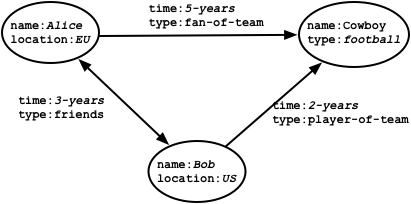
\includegraphics[scale=0.5]{./images/property-graph-model}
		\caption{Property Graph Model}
		\label{fig:property-graph-model-eng}
	\end{figure}

	\begin{itemize}
		\item The \textbf{nodes} contain \textbf{properties}. You can think of nodes as documents that group together a set of properties that define the characteristics of the document to which they belong.
		\item The \textbf{nodes} can be marked with one or more \textbf {labels}. Labels group nodes by similar characteristics or indicate the roles each plays in the data model.
		\item The \textbf{links} connect nodes to each other and define the structure of a graph. A link has an direction, a source node and a destination node.
		\item Like nodes, links can also have properties that add semantic value to the relationship.
		\item In all cases, the properties and their values can be used to restrict the results of searches performed in a graph.
	\end{itemize}

	Based on the theoretical model of tagged graphs discussed above, an implementation model was designed that will provide support to the data on which the recognition algorithms will act.

	The central element to be considered in the implementation model are the \textbf{nodes}. The nodes, in this area, model individual readings obtained by the observation instrument. Each node becomes equivalent, with this approach, to a record of the information exchange files. This process will be detailed in the section \ref{sec:sources-preprocessing}.
	
	A unique identifier will be generated for each node to simplify the queries and subsequent recovery of the information associated with them. There are some properties inherent to each of the observations that will be stored in the corresponding nodes, such as the coordinates of that observation, the section of the sky that is being surveyed and the settings of the observation instrument. All these characteristics are necessary to reconstruct the original observation conditions from the data.
	
	The \textbf {labels}, once the general data of each node is imported, will play a fundamental role since they are responsible for the storage of all the additional information that will be used in the searches.
	
	Among the possible values to be stored are the various readings taken by the instruments and optical processors of the telescopes from which the information is obtained, including readings in the optical spectrum as well as in the infrared or ultraviolet (identified with certain particular wavelengths), labels relating to brightness, rotation speed, nomenclature, etc. will also be incorporated.
	
	In the graph model the relations between the nodes are of crucial importance for the paths and are fundamental for the detection of patterns. But in the field under study it must be recognized that there is no single characteristic that links two stars and their associated readings.
	
	There are many parameters that can indicate relations, such as the distance between the stars, the luminosity, the size, the different spectral readings, their rotation period, etc. As it is impracticable to establish relationships for all possible combinations of characteristics, the implementation will allow generating those relationships on demand.
	
	That is, as a preliminary step to the analysis and detection of patterns, the user must indicate which feature or combination of them he wants to use to generate the relationships between the stars. Then the indicated relationships will be generated and the analysis will be made based on the resulting graph with the structure determined according to the characteristics indicated by the user.
	
	This approach has been used in a timely manner in the papers published by Coutinho et. al 2016 \cite{coutinho2016network}, an example of which is presented in Figure \ref{fig:galaxies-as-graph-eng}.
	
	\begin{figure}[h]
		\centering
		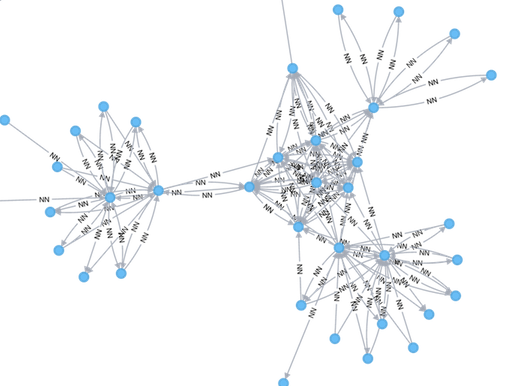
\includegraphics[width=0.7\linewidth]{./images/galaxies-graph-visualization-small}
		\caption{Galaxies as labeled graph. Coutinho et. al}
		\label{fig:galaxies-as-graph-eng}
	\end{figure}
	
	\subsection{Sources and pre-processing of data} \label{sec:sources-preprocessing}
	
	The aforementioned astronomical survey projects have large repositories of publicly accessible information, which are going to be used as sources of information to load the analysis database.
	
	The \emph{de facto} standard for the exchange of astronomical information is based on the FITS file format (Flexible Image Transport System\cite{hanisch2001definition}) which will be used as a basis for all data import routines.
	
	ONgDB, the database used in this work, has the possibility of importing data files in a massive way, which is very necessary because each one of the source files generally have volumes of approximately half a million records. For this, it uses comma separated files with a particular format.
	
	It is necessary to pre-process the information so that it is in an adequate format for its massive import into the database. To this end, a Python language development is proposed, which provides the AstroPy \cite{robitaille2013astropy} libraries that are suitable for the reading and parsing of FITS files and allows the CSV files to be managed with ease. The complete procedure is described in Figure \ref{fig:import-data-eng}.
	
	\begin{figure}[h]
		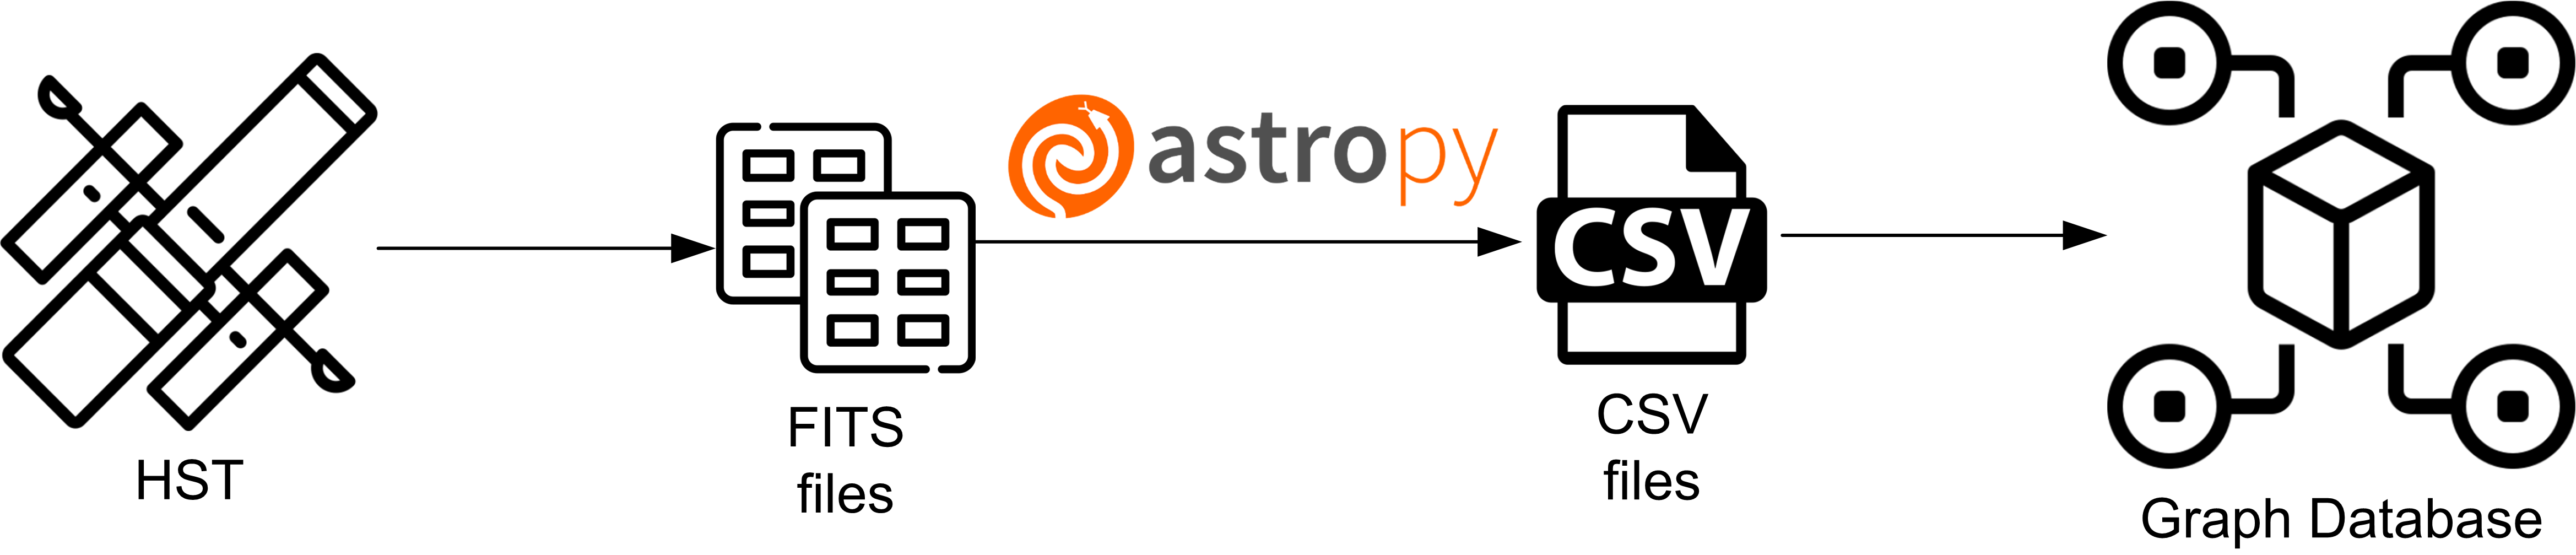
\includegraphics[width=\linewidth]{./images/importacion-datos}
		\caption{Data pre-processing and import flow}
		\label{fig:import-data-eng}
	\end{figure}

	\subsection{Selected storage}
	
	For the implementation of the data model we opted for the use of ONgDB (\url{https://www.graphfoundation.org/projects/ongdb/}), a completely Open Source alternative to Neo4J (\url{https://neo4j.com/}), which is perhaps the most widespread commercial graph database.
	
	We chose this product because it has some very valuable characteristics for the project:
	
	\begin{itemize}
		\item Natively represents the characteristics of the labeled graph model mentioned above
		\item Based on a commercial product of proven quality and updated technology
		\item It has a non-restrictive license that allows it to be used freely and free of charge in educational institutions and as part of research projects
		\item It has no restrictions regarding advanced features such as
		\begin{itemize}
			\item ACID Transactions
			\item Replication
			\item Monitoring
		\end{itemize}
	\end{itemize}
\else
	El auge de las actuales bases de datos de grafos nos brinda posibilidades importantes a la hora de modelar un dominio para el cual las bases de datos relacionales no tienen aplicación directa.
	
	La posibilidad de incluir en el esquema diseñado, información de tipos variados, sin penalizar por ellos las capacidades de búsqueda o la representatividad de la información es una de las características más favorables del modelo basado en grafos, lo que la hace especialmente recomendable en entornos en donde no se cuenta con un esquema establecido o no es estable o sufre fercuentes variaciones, ejemplos de esto son prototipos de diseño, bases de datos para la prueba de conceptos y almacenamientos para minería de datos\cite{robinson2015graph}.
	
	En términos de expresividad las bases de datos reducen la diferencia de impedancia entre el modelo de análisis y la implementación final, un problema que ha acosado a los diversos modelos de bases de datos desde hace muchos años.
	
	\subsection{Factores de representación}
	
	Para tener información relevante del dominio elegido y poder detectar patrones, se necesita contar con una base de grafos que represente la información de los cumulos estelares con la mayor exactitud posible.
	
	Actualmente se deben tener en cuenta al menos cuatro factores fundamentales a la hora de diseñar un sistema de representación del conocimiento en cualquier dominio dado\cite{van2008handbook}:
	
	\begin{itemize}
		\item \textbf{Adecuación Representacional:} Habilidad para representar todas las clases de conocimiento que son necesarias en el dominio.
		\item \textbf{Adecuación Inferencial:} Habilidad de manipular estructuras de representación de tal manera que devengan o generen nuevas estructuras que correspondan a nuevos conocimientos inferidos de los anteriores.
		\item \textbf{Eficiencia Inferencial:} Capacidad del sistema para incorporar información adicional a la estructura de representación, llamada metaconocimiento, que puede emplearse para focalizar la atención de los mecanismos de inferencia con el fin de optimizar los cómputos.
		\item \textbf{Eficiencia en la Adquisición:} Capacidad de incorporar fácilmente nueva información. Idealmente el sistema por sí mismo deberá ser capaz de controlar la adquisición de nueva información y su posterior representación.
	\end{itemize}
	
	Estos factores se tuvieron en cuenta durante el proceso de diseño de las estructuras de la base de datos, de manera tal que se puedan maximizar los resultados a la vez que se mantienen eficientes las operaciones de cómputo.
	
	\subsection{El modelo de grafos etiquetados}
	
	El enfoque propuesto en el presente trabajo se basa en el modelo de grafos etiquetados, existente en multitud de productos de base de datos de grafos, tanto comerciales como Open Source.
	
	Un \emph{grafo de propiedades etiquetadas} esta compuesto de nodos, relaciones, propiedades y etiquetas, tal como se puede apreciar en la Figura \ref{fig:property-graph-model}.
	
	\begin{figure}[h]
		\centering
		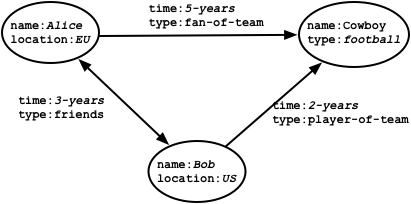
\includegraphics[scale=0.5]{./images/property-graph-model}
		\ifdefined\ingles
			\caption{Property Graph Model}
		\else
			\caption{Modelo de Grafo Etiquetado}
		\fi
		\label{fig:property-graph-model}
	\end{figure}
	
	
	\begin{itemize}
		\item Los \textbf{nodos} contienen \textbf{propiedades}. Se puede pensar en los nodos como documentos que agrupan un conjunto de propiedades que definen las características del documento al que pertenecen. 
		\item Los \textbf{nodos} pueden ser marcados con una o más \textbf{etiquetas}. Las etiquetas agrupan nodos por características similares o indican los roles que cada uno juega en el modelo de datos.
		\item Las \textbf{relaciones} conectan nodos entre si y definen la estructura de un grafo. Una relación tiene una dirección, un nodo de origen y un nodo de destino.
		\item Como los nodos las relaciones también pueden tener propiedades que le agregan valor semántico a la relación.
		\item En todos los casos, las propiedades y sus valores pueden utilizarse para restringir los resultados de las búsquedas realizadas en un grafo.
	\end{itemize}
	
	En base al modelo teórico de grafos etiquetados expuesto anteriormente se diseñó un modelo de implementación que brindará soporte a los datos sobre los que actuarán los algoritmos de reconocimiento.
	
	El elemento central a considerar en el modelo de implementación son los \textbf{nodos}. Los nodos, en este ámbito modelan lecturas puntuales obtenidas por el instrumento de observación. Cada nodo se hace equivalente, con este enfoque, a un registro de los archivos de intercambio de información. Este proceso se detallará en la sección \ref{sec:fuentes-preprocesamiento}.
	
	Se generará un identificador único para cada nodo para simplificar las consultas y posterior recuperación de la información asociada a los mismos. Existen algunas propiedades inherentes a cada una de las observaciones que serán almacenadas en los nodos correspondientes, como por ejemplo las coordenadas de dicha observación, la sección del cielo que se está relevando y los ajustes del instrumento de observación. Todas estas características son necesarias para reconstruir las condiciones originales de observación a partir de los datos.
	
	Las \textbf{etiquetas}, una vez importados los datos generales de cada nodo, pasarán a cumplir un rol fundamental ya que son las responsables del almacenamiento de toda la información adicional que se utilizará en las búsquedas.
	
	Dentro de los posibles valores a almacenar se encuentran las diversas lecturas tomadas por los instrumentos y procesadores ópticos de los telescopios de dónde se obtiene la información, incluyendo lecturas en el espectro óptico así como en el infrarrojo o ultravioleta (identificados con ciertas longitudes de onda particulares), también se incorporarán etiquetas relativas a luminosidad, velocidad de rotación, nomenclatura, etc.
	
	En el modelo de grafos las relaciones entre los nodos son de crucial importancia para los caminos y son fundamentales para la detección de patrones. Pero en el ámbito bajo estudio hay que reconocer que no existe una única característica que relaciones dos estrellas y sus lecturas asociadas.
	
	Existen multitud de parámetros que pueden indicar relaciones, tales como la distancia entre las estrellas, la luminosidad, el tamaño, las diferentes lecturas espectrales, su período de rotación, etc. Como es impracticable establecer relaciones para todas las posibles combinaciones de características, la implementación permitirá generar dichas relaciones a demanda.
	
	Es decir, como paso previo al análisis y detección de patrones, el usuario deberá indicar qué característica o combinación de ellas quiere utilizar para generar las relaciones entre las estrellas. Acto seguido se generarán las relaciones indicadas y el análisis se realizará en base a el grafo resultante con la estructura determinada de acuerdo a las características indicadas por el usuario.
	
	Dicho enfoque se ha utilizado oportunamente en los trabajos publicados por Coutinho et. al 2016\cite{coutinho2016network}, un ejemplo de lo cual se presenta en la Figura \ref{fig:galaxies-as-graph}.
	
	\begin{figure}[h]
		\centering
		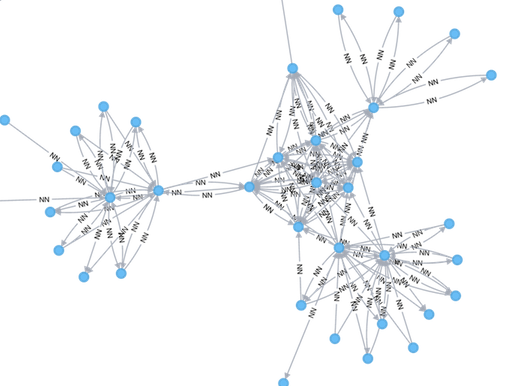
\includegraphics[width=0.7\linewidth]{./images/galaxies-graph-visualization-small}
		\ifdefined\ingles
			\caption{Galaxies as labeled graph. Coutinho et. al}
		\else
			\caption{Galaxias representadas como grafo etiquetado. Coutinho et. al}
		\fi
		\label{fig:galaxies-as-graph}
	\end{figure}
	
	
	\subsection{Fuentes y pre-procesamiento de los datos}\label{sec:fuentes-preprocesamiento}
	
	Los mencionados proyectos de survey astronómicos cuentan con grandes repositorios de información accesible de forma pública, los cuales van a ser utilizados como fuentes de información para cargar la base de datos de análisis.
	
	El estandar de facto para el intercambio de información astronómica se basa en el formato de archivos FITS (Flexible Image Transport System\cite{hanisch2001definition}) el cual será utilizado como base para todas las rutinas de importación de datos.
	
	ONgDB cuenta con la posibilidad de importar archivos de datos de forma masiva, lo cual es muy necesario debido a que los archivos fuente generalmente cuentan con volúmenes de aproximadamente medio millón de registros. Para ello utiliza archivos separados por comas con un formato particular 
	
	Es necesario realizar un procesamiento previo de la información para que la misma se encuentre en un formato adecuado para su importación masiva en la base de datos. Para ello se propone un desarrollo en lenguaje Python, el cual provee las librerías AstroPy\cite{robitaille2013astropy} que son adecuadas para la tarea de lectura y parseo de los archivos FITS y permite gestionar con cierta facilidad los archivos CSV de destino. El procedimiento completo está descripto en la Figura \ref{fig:importacion-datos}.
	
	\begin{figure}[h]
		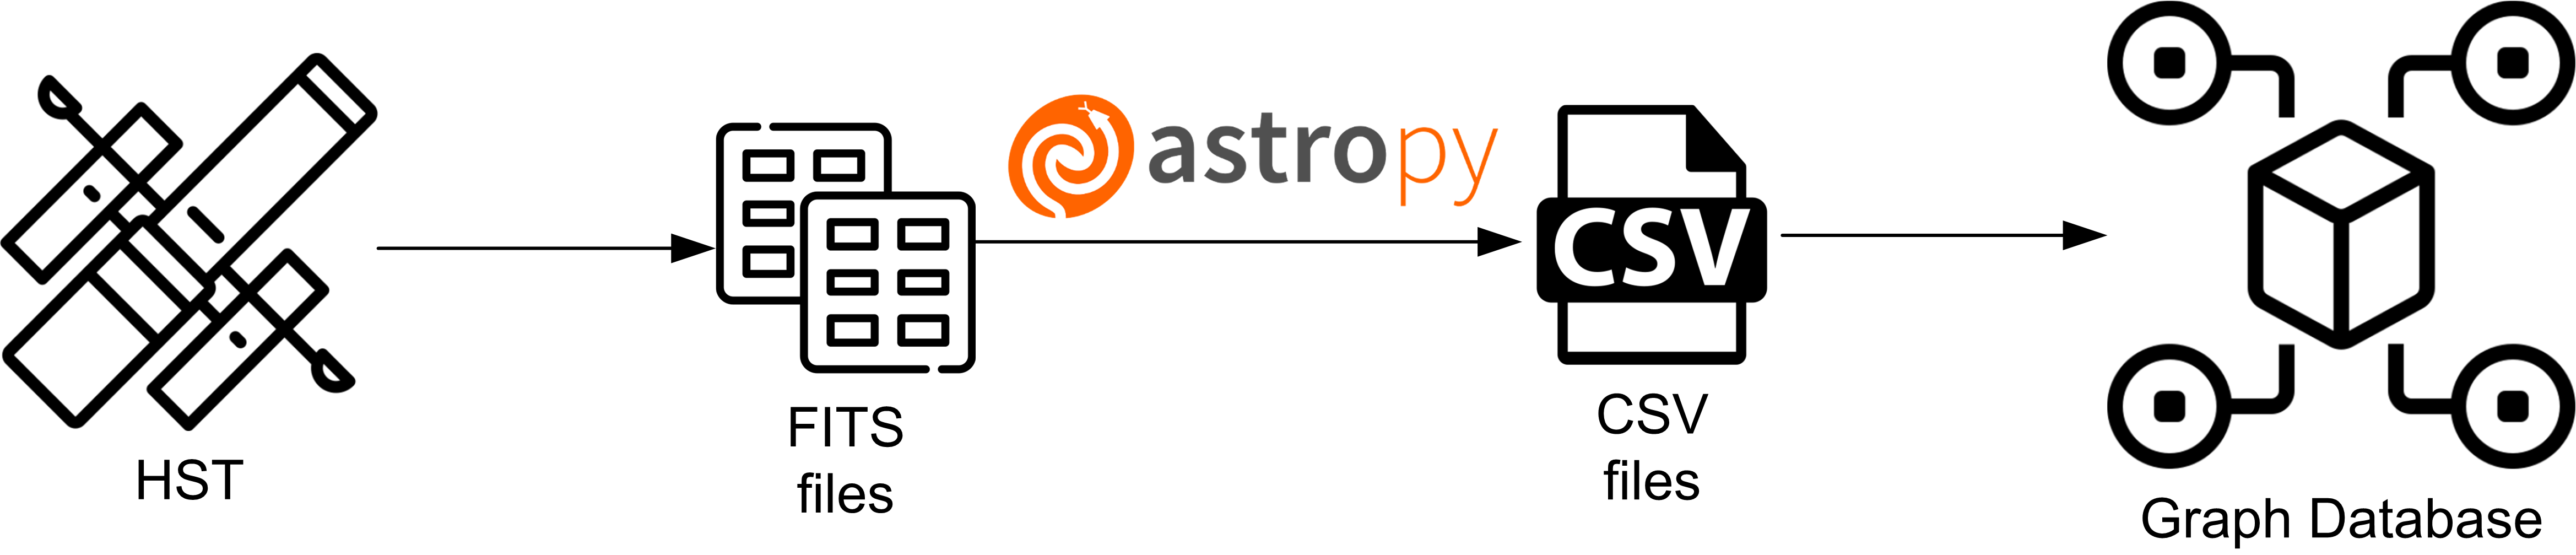
\includegraphics[width=\linewidth]{./images/importacion-datos}
		\ifdefined\ingles
		\caption{Data pre-processing and import flow}
		\else
		\caption{Pre-procesamiento e importación de datos}
		\fi
		\label{fig:importacion-datos}
	\end{figure}
	
	\subsection{El almacenamiento seleccionado}
	
	Para la implementación del modelo de datos se optó por la utilización de ONgDB (\url{https://www.graphfoundation.org/projects/ongdb/}), una alternativa completamente Open Source a Neo4J (\url{https://neo4j.com/}), la que quizá sea la base de datos de grafos comercial más difundida.
	
	Se optó por este producto debido a que reúne algunas características muy valiosas para el proyecto:
	
	\begin{itemize}
		\item Representa de forma nativa las características del modelo de grafo etiquetado mencionado anteriormente
		\item Se basa en un producto comercial de probada calidad y tecnología actualizada
		\item Dispone de una licencia no restrictiva que permite utilizarlo de manera libre y gratuita en instituciones educativas y como parte de proyectos de investigación
		\item No tiene restricciones en cuanto a características avanzadas tales como
		\begin{itemize}
			\item Transacciones ACID
			\item Replicación
			\item Monitoreo
		\end{itemize}
	\end{itemize}
	
	%\subsection{El diseño físico de la base de datos}
	%
	%ESTA SECCION NO SE SI TIENE MUCHO SENTIDO, NO DICE MUCHO, YO LA PUSE EN FUTURO PORQUE NO DICE NADA DE COMO ESTA DISEÑADA LA BASE DE DATOS
	%SI LA DEJAS YO LA PONDRÍA ANTES DE LA SECCION DE ALMACENAMIENTO SELECCIONADO
	%
	%El diseño físico de la base de datos de grafos subyacente para el análisis y detección de patrones tiene un impacto directo y decisivo en el tipo y variedad de los algoritmos que se pueden utilizar y en el rendimiento general del sistema. 
	%
	%Este diseño debería balancear dos elementos importantes, que muchas veces se contraponen. Por una parte el diseño debería ser lo suficientemente genérico y flexible como para permitir representar las lecturas astronómicas actualmente disponibles, como permitir la incorporación futura de nuevos valores, adecuar los formatos de archivos de importación o incluir metadatos necesarios para el análisis.
	%
	%Por otra parte las estructuras deberían permitir la utilización de diversos algoritmos, establecidos y probados, de una forma eficiente, así como debería dar la posibilidad de desarrollar, probar e implementar algoritmos desarrollados para los usos específicos mencionados en el presente trabajo.
	%
	%Estas dos necesidades contrapuestas obligan a plantear algunas soluciones de compromiso y a utilizar todos los mecanismos específicos presentes en el motor de base de datos elegido (ONgDB) para mantener un rendimiento aceptable sin sacrificar flexibilidad.
\fi	


\section{
\ifdefined\ingles	
	Conclusions and future work
\else
	Conclusiones y trabajos futuros
\fi
}
\ifdefined\ingles	

	In view of the results obtained during the elaboration of this work, it is considered that the graph databases are a valid mechanism for the storage of astronomical information, providing a flexible scheme but that at the same time can query efficiently large volumes of data.
	
	The labeled graphs allow to accurately reflect the astronomical data, also allowing the growth and adaptation of the structures according to the needs that arise from the data files, a task that is difficult in the case of using relational databases.
	
	In subsequent stages during the evolution of the thesis plan, it is expected to optimize the mechanisms for importing astronomical information and provide users with some intuitive tools to perform both the data import tasks and the definition of the criteria for the generation of relationships demand.
	
	An end user query system will be developed to indicate the parameters to be used in the searches and a module will be implemented that obtains some relevant statistical indicators according to the stored data.
	
	Subsequently, some pattern models existing in other disciplines will be analyzed and tests will be implemented to use these patterns in an astronomical environment. The purpose of this activity is to determine if there are pre-existing patterns that have application in an area for which they have not been designed. Of special interest are the small-world network algorithms\cite{kleinberg2000navigation} and the social network algorithms\cite{carrington2005models}.

\else

	En vista a los resultados obtenidos durante la elaboración del presente trabajo se considera que las bases de datos de grafos son un mecanismo válioso para el almacenamiento de información astronómica, brindando un esquema flexible pero que a la vez puede realizar consultas de manera eficiente en grandes volúmenes de datos.
	
	Los grafos etiquetados permiten reflejar con exactitud los datos astronómicos, permitiendo asimismo el crecimiento y adecuación de las estructuras de acuerdo a las necesidades que surjan a partir de los archivos de datos, tarea ésta que es dificultosa en el caso de utilizar bases de datos relacionales.
	
	En posteriores etapas durante la evolución del plan de tesis se prevé optimizar los mecanismos de importación de información astronómica y brindar a los usuarios algunas herramientas intuitivas para realizar tanto las tareas de importación de datos como la definición de los criterios para la generación de las relaciones a demanda.
	
	Se desarrollará un sistema de consulta que permita indicar los parámetros a utilizar en las búsquedas y se implementará un módulo que obtenga algunos indicadores estadísticos relevantes de acuerdo a los datos almacenados.
	
	Posteriormente se analizarán algunos modelos de patrones existentes en otras disciplinas y se implementarán tests para utilizar dichos patrones en un ámbito astronómico. La finalidad de ésta actividad es determinar si existen patrones pre-existentes que tengan aplicación en un ámbito para el que no han sido diseñados. Un especial interés tienen los algoritmos de redes de mundo pequeño\cite{kleinberg2000navigation} y los algoritmos de redes sociales\cite{carrington2005models}.

\fi

%\setcounter{tocdepth}{1}
%\listoftodos

% Material CITADO, entra bajo el titulo REFERENCIAS
%\defbibnote{bibnote}{\emph{El presente material bibliográfico se ha utilizado como material de estudio pero no se ha citado directamente en el texto.}}

\printbibliography[category=cited]

% Material NO CITADO, entra bajo el titulo BIBLIOGRAFÍA ADICIONAL
%\section*{Bibliografía adicional (no citada)}
%\printbibliography[heading=bibempty,title={Bibliografí­a adicional}, prenote=bibnote, notcategory=cited, resetnumbers=true, omitnumbers]

\end{document}
